\documentclass[a4paper]{article}
\usepackage[english]{babel}
\usepackage[top=2cm,bottom=3cm,left=2.5cm,right=2.5cm]{geometry}
\usepackage[colorlinks=true, allcolors=black]{hyperref}
\usepackage{wrapfig} %문단 내 이미지 삽입
\usepackage[abs]{overpic} %이미지 위 텍스트 삽입
\usepackage{graphicx} %색상
\usepackage{mdframed} %글상자
\usepackage{titlesec} %섹션 이름 변경
\titlespacing*{\section}{0mm}{0mm}{0mm}
\titleformat{\section}{\bfseries\Large}{\Huge{\color{blue!60!green!80}\thesection}}{2ex}{}[]
\titlespacing*{\subsection}{0mm}{0mm}{0mm}
\titleformat{\subsection}{\bfseries}{\thesubsection\hspace{1ex}|}{1ex}{}[]
\usepackage[many]{tcolorbox}
\newcommand{\asw}[2]{
	\begin{flushright}
		{\color{blue!60!green}#1 \quad #2 \quad $\blacktriangleleft$}
	\end{flushright}
}
\newcommand{\pbox}[3]
{
	\begin{tcolorbox}[
		boxsep = 0mm,
		left = 3mm,
		right = 3mm,
		valign = center,
		colupper = black,
		colback = #1!70!black!15,
		colframe = #1!65!black,
		segmentation style = {
			double = #1!65!black,
			draw = #1!65!black,
			double distance=0.2mm,
			solid},
		after skip = 0mm
		]
		{\color{#1!65!black}#2}
		\ifx#3""\else\tcbline #3\fi
	\end{tcolorbox}
}
\newcommand{\cabox}[2]{\pbox{orange}{#1}{#2}}
\newcommand{\spbox}[2]{\pbox{green}{#1}{#2}}
\newcommand{\prbox}[2]{\pbox{blue!white!80}{#1}{#2}}
\newcommand{\lpbox}[2]{\pbox{magenta}{#1}{#2}}

\newcommand{\secbox}[1]{
	\begin{tcolorbox}[
		boxsep = 0mm,
		left = 4mm,
		right = 4mm,
		valign = center,
		colupper = blue!70!green!90,
		colback = blue!70!green!15,
		colframe = white,
		boxrule = 0mm
		]
		#1
	\end{tcolorbox}
}
\usepackage{amsmath, amsfonts, amssymb, bm} %수식
	\DeclareMathOperator{\arccsc}{arccsc}
	\DeclareMathOperator{\arcsec}{arcsec}
	\DeclareMathOperator{\arccot}{arccot}
	\DeclareMathOperator{\csch}{csch}
	\DeclareMathOperator{\sech}{sech}
	\DeclareMathOperator{\arcsinh}{arcsinh}
	\DeclareMathOperator{\arccosh}{arccosh}
	\DeclareMathOperator{\arctanh}{arctanh}
	\DeclareMathOperator{\arccsch}{arccsch}
	\DeclareMathOperator{\arcsech}{arcsech}
	\DeclareMathOperator{\arccoth}{arccoth}

	\DeclareMathOperator{\meter}{m}
	\DeclareMathOperator{\cm}{cm}
	\DeclareMathOperator{\mm}{mm}
	\DeclareMathOperator{\mum}{\mu m}
	\DeclareMathOperator{\newton}{N}
	\DeclareMathOperator{\kn}{kN}
	\DeclareMathOperator{\kgf}{kgf}
	\DeclareMathOperator{\pa}{Pa}
	\DeclareMathOperator{\kpa}{kPa}
	\DeclareMathOperator{\mpa}{MPa}
	\DeclareMathOperator{\gpa}{GPa}
	\DeclareMathOperator{\knpm}{kN/m}
	\DeclareMathOperator{\kph}{km/h}
	\DeclareMathOperator{\mps}{m/s}
	\DeclareMathOperator{\tkph}{kph}
	\DeclareMathOperator{\tmps}{mps}
	\DeclareMathOperator{\mpss}{m/s^2}
	\DeclareMathOperator{\dgr}{\!^\circ}
	\DeclareMathOperator{\cel}{\!^\circ C}
	\DeclareMathOperator{\kg}{kg}
	\DeclareMathOperator{\kgpcm}{kg/m^3}
	\DeclareMathOperator{\nm}{N\cdot m}
	\DeclareMathOperator{\kw}{kW}
	\DeclareMathOperator{\kwh}{kWh}
	\DeclareMathOperator{\mmhg}{mmHg}
	\DeclareMathOperator{\snd}{s}
\usepackage{polynom} %나눗셈 필산
\usepackage{cancel} %수식 약분선
\usepackage[normalem]{ulem}%취소선
\usepackage{array} %표
\usepackage{kotex} %한글

\title{
	\vspace{150pt}
	\textbf{\Huge Solutions}\\[10pt]
	of the Dynamics Final Exam 2023-1\\[20pt]
	\vspace{55pt}
	}
\author{E.Hong\vspace{90pt}}
\date{\today}

\begin{document}

\maketitle
\setlength{\parindent}{3mm}

\begin{center}
	\includegraphics[width=0.45\textwidth]{SSU symbol KR-EN.jpg}
\end{center}

\newpage

\spbox{\subsection*{Question 1}}
	{
	\begin{tabular}{m{75mm}m{70mm}}
	\includegraphics{img/q01.png}
		& The 2-kg sub-satellite $B$ has an initial velocity $\mathbf{v}_B = 3\mps \mathbf{j}$. It is connected to the 20-kg base-satellite $A$ by a 500-m space tether. Determine the velocity of the base satellite and sub-satellite immediately after the tether becomes taut (assuming no rebound).
	\end{tabular}
	}
	\vspace{\baselineskip}
	\hspace{20mm}\includegraphics{img/q01-1.png}
	\begin{align*}
		&\frac{m_Bv_B}{5} = \frac{m_Av_A' + m_Bv_A'}{4} = \frac{\sqrt{(m_Bv_B')^2 - (m_Bv_A')^2}}{3}\\
		&\left\{\begin{array}{l}
			4m_Bv_B = 5v_A'(m_A + m_B)\\[5pt]
			3v_B = 5\sqrt{v_B'^2 - v_A'^2}
		\end{array}\right.\\
		&v_A' = \frac{4m_Bv_B}{5(m_A + m_B)} = \frac{4(2)(3)}{5(20 + 2)}\mps = \frac{12}{55}\mps = 0.218\mps\\
		&v_B' = \sqrt{\frac{9}{25}v_B^2 + v_A'^2} = \sqrt{\frac{9}{25}(3)^2 + \left(\frac{12}{55}\right)^2}\mps = 1.813\mps\\
		&\theta_A = \arctan\frac{400\meter}{300\meter} = \arctan\frac{4}{3} = 53.1\dgr\\
		&\theta_B = \theta_A + \arccos\frac{v_A'}{v_B'} = 53.1\dgr + \arccos\frac{0.218}{1.813} = 136.2\dgr
	\end{align*}
	\asw{}{$\mathbf{v}_A = 0.218\mps\measuredangle 53.1\dgr$}
	\asw{}{$\mathbf{v}_B = 1.813\mps\measuredangle 136.2\dgr$}
	
	
\newpage

\spbox{\subsection*{Question 2}}
	{
		\begin{tabular}{m{40mm}m{105mm}}
			\includegraphics{img/q02.png}
			& A 20-kg block $B$ is suspended from a 2-m cord attached to a 30-kg cart $A$, which may roll freely on a frictionless, horizontal track. If the system is released from rest in the position shown, determine the velocities of $A$ and $B$ as $B$ passes directly under $A$.
		\end{tabular}
	}
	\vspace{\baselineskip}
	\noindent Let the state 1 be the initial state and the state 2 be when $B$ passes directly under $A$.
	\begin{align*}
		&\cancelto{0}{T_1} + V_{g1} = T_2 + \cancelto{0}{V_{g2}}\\
		&m_Bgl(1-\cos25\dgr) = \frac{1}{2}m_Av_A^2 + \frac{1}{2}m_Bv_B^2\\
		&m_Av_A^2 + m_Bv_B^2 = 2m_Bgl(1-\cos25\dgr)\tag{1}
	\end{align*}
	\noindent Impulses by gravity and ground are independent to horizontal component of momentum of $A$ and $B$.
	\begin{align*}
		&\sum p_{x1} = \sum p_{x2}\\
		&0 = -m_Av_A + m_Bv_B\tag{2}\\
		&\left\{\begin{array}{l}
			m_Av_A^2 + m_Bv_B^2 = 2m_Bgl(1-\cos25\dgr)\\[5pt]
			-m_Av_A + m_Bv_B = 0
		\end{array}\right.\tag{1 \& 2}\\
		&m_Av_A = m_Bv_B\\
		&m_Am_Bv_A^2 + m_A^2v_A^2 = 2m_B^2gl(1-\cos25\dgr)\\
		&\frac{m_A}{m_B}v_A^2 + \left(\frac{m_A}{m_B}\right)^2v_A^2 = 2gl(1-\cos25\dgr)\\
		&k(k+1)v_A^2 = 2gl(1-\cos25\dgr),\qquad k = \frac{m_A}{m_B} = 1.5\\
		&v_A = \sqrt{\frac{2gl(1-\cos25\dgr)}{k(k+1)}} = \sqrt{\frac{2(9.81)(2)(1-\cos25\dgr)}{(1.5)(2.5)}}\mps = 0.990\mps\\
		&v_B = \frac{m_A}{m_B}v_A = kv_A = (1.5)(0.990)\mps = 1.485\mps
	\end{align*}
	\asw{}{$\mathbf{v}_A = 0.990\mps\leftarrow$}
	\asw{}{$\mathbf{v}_B = 1.485\mps\rightarrow$}


\newpage

\spbox{\subsection*{Question 3}}
{
	A crank $AB$ is rotating clockwise with constant angular speed $900\,\mathrm{rpm}$. Determine the acceleration of piston $P$ when $\theta = 120\dgr$.
}
	\vspace{\baselineskip}
	\includegraphics{img/q03.png}\hspace{20mm}\includegraphics{img/q03-1.png}
	\vspace{\baselineskip}
	\begin{align*}
		&L = 0.15\meter,\quad l = 0.05\meter\\
		&\dot{\theta} = 900\,\mathrm{rpm}\times\frac{1\,\mathrm{min}}{60\snd}\times\frac{2\pi\,(\mathrm{rad})}{1\,\mathrm{rev}} = 30\pi\snd^{-1}\\
		&\frac{\sin(\pi-\theta-\beta)}{50\mm} = \frac{\sin\theta}{150\mm}\\
		&\sin(\theta+\beta) = \frac{1}{3}\sin\theta\\
		&\phi = \theta + \beta - \frac{\pi}{2}\\
		&\sin\left(\phi + \frac{\pi}{2}\right) = \frac{1}{3}\sin\theta\\
		&3\cos\phi = \sin\theta\\
		&\phi = \arccos\left(\frac{\sin\theta}{3}\right) = \arccos\left(\frac{\sin120\dgr}{3}\right) = 73.2213\dgr\\
		&-3\dot{\phi}\sin\phi = \dot{\theta}\cos\theta\\
		&\dot{\phi} = -\frac{\dot{\theta}\cos\theta}{3\sin\phi} = -\frac{(30\pi\snd^{-1})\cos120\dgr}{3\sin73.2213\dgr} = 16.40644\snd^{-1}\\
		&-3\ddot{\phi}\sin\phi-3\dot{\phi}^2\cos\phi = - \dot{\theta}^2\sin\theta\qquad\left(\because \ddot{\theta} = 0\right)\\
		&\ddot{\phi} = \frac{- \dot{\theta}^2\sin\theta + 3\dot{\phi}^2\cos\phi}{-3\sin\phi} = \frac{-(30\pi\snd^{-1})^2\sin120\dgr + 3(16.40644\snd^{-1})^2\cos120\dgr}{-3\sin73.2213\dgr} = 2597.06\snd^{-2}\\
		&a_B = l\dot{\theta}^2\\
		&a_{D/B,r} = -L\dot{\phi}^2\\
		&a_{D/B,\theta} = L\ddot{\phi}\\
		&\mathbf{a}_D = \mathbf{a}_{D/B} + \mathbf{a}_B\\
		&a_{D} = a_{D/B,r}\sin\phi + a_{D/B,\theta}\cos\phi + a_B\cos\theta = -L\dot{\phi}^2\sin\phi + L\ddot{\phi}\cos\phi + l\dot{\theta}^2\sin\left(\theta - \frac{\pi}{2}\right)\\
		&\qquad = -(0.15)(16.40644)^2\sin73.2213\dgr + (0.15)(2597.06)\cos73.2213\dgr + (0.05)(30\pi)^2\sin30\dgr\\
		&\qquad = 296\mpss
	\end{align*}
	\asw{}{$296\mpss\uparrow$}

\newpage

\spbox{\subsection*{Question 4}}
{
	\begin{tabular}{m{45mm}m{100mm}}
		\includegraphics{img/q04.png}
		& At the instant shown the length of the boom $AB$ is being increased at the constant rate of $0.2\mps$, the boom is being lowered at the constant rate of $0.08\,\mathrm{rad/s}$, and it is moving forward with a speed of $0.1\mps$ and is slowing down at $0.05\mpss$. Determine ($a$) the velocity of Point $B$, ($b$) the acceleration of Point $B$.
	\end{tabular}
}
	\vspace{\baselineskip}
	\begin{align*}
		&r = 6\meter,\quad \dot{r} = 0.2\mps,\quad \ddot{r} = 0,\\
		&V = 0.1\mps,\quad  \dot{V} = -0.05\mpss\\
		&\theta = 30\dgr,\quad \dot{\theta} = - 0.08\snd^{-1},\quad \ddot{\theta} = 0\\
		&v_{B/A,r} = \dot{r},\quad v_{B/A,\theta} = r\dot{\theta}\\
		&v_{B,x} = \dot{r}\cos\theta - r\dot{\theta}\sin\theta + V = (0.2)\cos30\dgr - (6)(-0.08)\sin30\dgr + 0.1\,[\mps] = 0.513\mps\\
		&v_{B,y} = \dot{r}\sin\theta + r\dot{\theta}\cos\theta = (0.2)\sin30\dgr + (6)(-0.08)\cos30\dgr\,[\mps] = -0.316\mps\\
		&v_B = \sqrt{v_{B,x}^2 + v_{B,y}^2} = 0.603\mps\\
		&\phi_v = \arctan\frac{v_{B,y}}{v_{B,x}} = -31.6\dgr
	\end{align*}
	\asw{($a$)}{$0.603\mps\measuredangle -31.6\dgr$}
	\begin{align*}
		&a_{B/A,r} = \ddot{r} - r\dot{\theta}^2 = - r\dot{\theta}^2,\quad a_{B/A,\theta} = r\ddot{\theta} + 2\dot{r}\dot{\theta} = 2\dot{r}\dot{\theta}\\
		&a_{B,x} = -r\dot{\theta}^2\cos\theta - 2\dot{r}\dot{\theta}\sin\theta + \dot{V} = -(6)(-0.08)^2\cos30\dgr - 2(0.2)(-0.08)\sin30\dgr - 0.05\,[\mpss]\\
		&\qquad = -0.0672554\mpss\\
		&a_{B,y} = -r\dot{\theta}^2\sin\theta + 2\dot{r}\dot{\theta}\cos\theta = -(6)(-0.08)^2\sin30\dgr + 2(0.2)(-0.08)\cos30\dgr\,[\mpss]\\
		&\qquad = -0.0469128\mpss\\
		&a_B = \sqrt{a_{B,x} + a_{B,y}} = 0.0820\mpss\\
		&\phi_a = \arctan\frac{a_{B,y}}{a_{B,x}} = 34.9\dgr
	\end{align*}
	\asw{($b$)}{$0.0820\mpss\measuredangle -145.1\dgr$}
	
\newpage

\spbox{\subsection*{Question 4 | Alternative Solution}}{}
	\vspace{10pt}
	The system $xy$ on point $A$. The system $XY$ is fixed framed.
	\begin{align*}
		&\mathbf{r}|_A = \mathbf{r}|_{xy} = 6\mathbf{e}_r\meter,\quad \dot{\mathbf{r}}|_{xy} = 0.2\mathbf{e}_r\mps = \text{const.} \quad\Rightarrow\quad \ddot{\mathbf{r}}|_{xy} = \mathbf{0}\\
		&\dot{\mathbf{r}}_A = 0.1\mathbf{i}\mps,\quad \ddot{\mathbf{r}}_A = -0.05\mathbf{i}\mpss\\
		&\theta = 30\dgr,\quad \mathbf{e}_r = \cos\theta\mathbf{i} + \sin\theta\mathbf{j},\quad \bm{\Omega} = -0.08\mathbf{k}\snd^{-1} = \text{const.} \quad\Rightarrow\quad \dot{\bm{\Omega}} = \mathbf{0}\\
		&\dot{\mathbf{r}}|_{XY} = \dot{\mathbf{r}}_A + \dot{\mathbf{r}}|_A = \dot{\mathbf{r}}_A + \dot{\mathbf{r}}|_{xy} + \bm{\Omega}\times\mathbf{r}|_A\\
		&\qquad = (0.1)(\rightarrow) + (0.2)\measuredangle30\dgr + (0.08\cdot6)\measuredangle (-60\dgr)\;[\mps]\\
		&\qquad = \left\{0.1 + 0.2\cos30\dgr + (0.08)(6)\cos(-60\dgr)\right\}\mathbf{i} + \left\{0.2\sin30\dgr + (0.08)(6)\sin(-60\dgr)\right\}\mathbf{j}\;[\mps]\\
		&\qquad = \left(0.513205\mathbf{i} - 0.315692\mathbf{j}\right)\mps\\
		&\left|\dot{\mathbf{r}}|_{XY}\right| = \sqrt{0.513205^2 + 0.315692^2}\mps = 0.603\mps\\
		&\theta_{v} = -\arctan\frac{0.315692}{0.513205} = -31.6\dgr
	\end{align*}
	\asw{($a$)}{$0.603\mps\measuredangle-31.6\dgr$}
	\begin{align*}
		&\ddot{\mathbf{r}}|_{XY} = \ddot{\mathbf{r}}_A + \cancelto{0}{\ddot{\mathbf{r}}|_{xy}} + \bm{\Omega}\times\left(\bm{\Omega}\times\mathbf{r}|_A\right) + \cancelto{0}{\dot{\bm{\Omega}}\times\mathbf{r}|_A} + 2\bm{\Omega}\times\dot{\mathbf{r}}|_{xy}\\
		&\qquad = (0.05)(\leftarrow) + (6)(0.08)^2\measuredangle(-150\dgr) + 2(0.08)(0.2)\measuredangle(-60\dgr)\;[\mpss]\\
		&\qquad = \left\{-0.05+(6)(0.08)^2\cos(-150\dgr) + 2(0.08)(0.2)\cos(-60\dgr)\right\}\mathbf{i}\\
		&\qquad\qquad\qquad + \left\{(6)(0.08)^2\sin(-150\dgr) + 2(0.08)(0.2)\sin(-60\dgr)\right\}\mathbf{j}\;[\mpss]\\
		&\qquad = (-0.0672554\mathbf{i} - 0.0469128\mathbf{j})\mpss\\
		&\left|\ddot{\mathbf{r}}|_{XY}\right| = \sqrt{0.0672554^2 + 0.0469128^2}\mps = 0.0820\mps\\
		&\theta_{a} = \arctan\frac{0.0469128}{0.0672554}-180\dgr = -145.1\dgr
	\end{align*}
	\asw{($b$)}{$0.0820\mpss\measuredangle -145.1\dgr$}



\end{document}